\chapter{Introduction}
\label{cha:introduction}

The main objective of the presented project is the implementation of parts of 3D engine in a browser environment. Parts of the engine are analysed side-by-side with a parallel engine compiled from C++. The objective of the analysis is to compare performance and describe possible issues related to the limited browser resources and dynamic features of JavaScript.

At the moment of writing, the majority of games are developed with C++ and usually DirectX. These technologies are mature and have excellent performance. Features of the language give flexibility and high-level solutions to effectively manage application (e.g. operator overloading, multiple inheritance) and enable to fine-tune the internals of application to achieve best execution times. For games with high budget\cite{gta} C++ is an obvious choice for having the best possible result.

However, in parallel to the AAA game industry, the casual and independent games sector is growing. In 2013, the market is expected to be worth \$8.64 billions in total. A total of 2.4 billion tablets and smartphones with casual games capabilities will be reached before the end of 2013. These games are less focused on creating cutting edge graphics and physics simulations and more on overall experience and social interactions.

JavaScript is a scripting language not designed to perform high-load computations. However, at present it is the only language widely supported by all browsers. With all it's advantages and quirks is the only choice available for programmers.\footnote{Currently two new languages are being developed -- Dart by Google and TypeScript by MicroSoft. However, to enable cross-compilation to JavaScript, the paradigm of these languages is similar and work is focused mainly on better IDE support.}

While suffering from design issues, JavaScript provides a complete environment that makes development very easy for both beginner and advanced programmers. Two very important components of every application are provided out of the box -- a rendering system and networking in the browser. They were designed for HTML pages to carry mainly text information, they are still suitable for gaming. Building a simple 2D game is often a matter of few hundred lines of code responsible for transferring user input to the positions of sprites defined in CSS. This is clearly visible during competitions like JS13kGames\cite{js13kgames} where all game assets and the code have to be fitted into 13kB package.

Many projects varying from server side solutions\cite{nodejs,coder} to hardware developer boards\cite{espruino} are taking advantage of this simplicity. From the perspective of game development, it is unlikely at the time of writing that an AAA game may be created to run in the browser. However, growing segments of casual, independent and social games are already targeting the web as a platform.

\section{Influence on the distribution process}

Traditionally, games are often still sold in actual boxes and some update system is always incorporated to patch any bugs appearing after initial release. Systems like Steam\cite{steam} are making this process easier, but still suffer from the necessity of having to install a game on the hard drive.

Creating an application that works in the browser simplifies distribution significantly. All assets and code are downloaded each time the user enters a website, so no update system is necessary -- all users are always playing the latest version. Usually browser games are monetised differently to traditional titles. Playing a basic version is usually free and earnings come from either ads or premium content. This is completely new approach, present also in MMO\footnote{Massive Multiplayer Online} games. It resulted in psychological research on leveraging compulsive behaviours to maximise profits\cite{exploitative-game-design}.

Working in a browser gives access to all social networks of users, so usage of Twitter or Facebook based features is very simple -- which boosts the promotion of the game. It also enables, though morally questionable, to target people who are not able to install games on company issued computers. Disallowing games in browsers is a far more complicated task for administrator, similar to blocking ads or mature content.

Lastly, the web is better suited to run easily on all platforms. The browser is a layer of abstraction that is transparent for the application, whether it runs on any traditional operating system, gaming console or mobile device. Of course performance and screen size should be taken into consideration, but ability to write one codebase that runs on multiple devices has already encouraged projects that package JavaScript applications as native ones\cite{phonegap}, greatly reducing development costs for the growing variety of phones and tablets.

\begin{figure}[h!]
  \caption{Game created with ImpactJS}
  \label{img:impactjs}
  \centering
	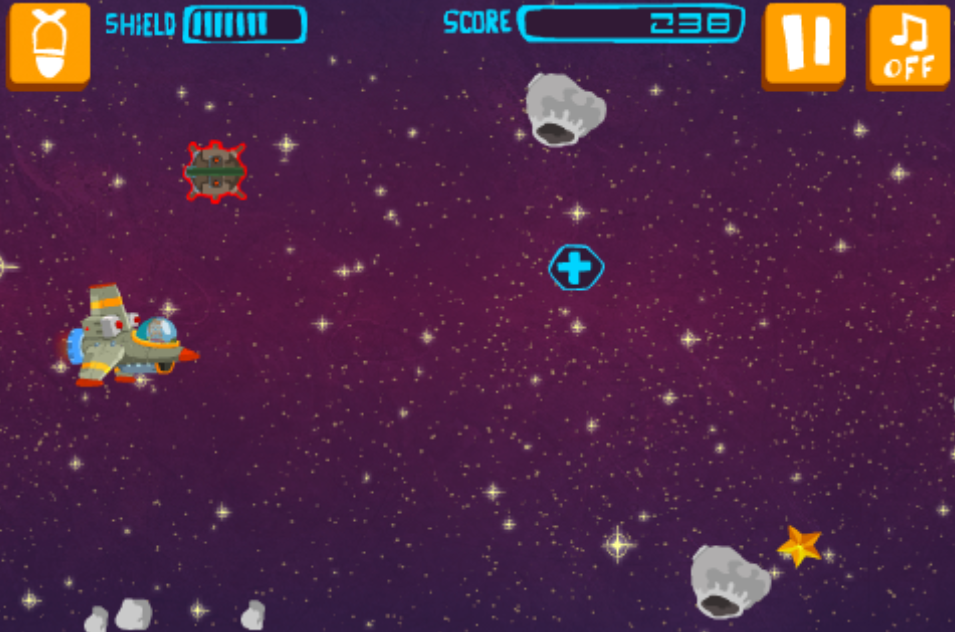
\includegraphics[width=12cm]{summary/impactjs.png}
\end{figure}

Multiple open-source and commercial game engines are being created lately. Examples worth mentioning are ImpactJS\cite{impactjs}, Turbulenz\cite{turbulenz} and Isogenic Engine\cite{isogenicengine}.


\begin{figure}[h!]
  \caption{Game created with Isogenic Engine}
  \label{img:isogenic}
  \centering
	
\includegraphics[width=12cm]{summary/isogenic.png}
\end{figure}

A very important and growing sector is interactive 3D arts with two major targets -- music videos and commercials. They are uniquely available only in browsers as a very viral extensions of regular marketing. One of the first occurrences of this technology was the video for Rome music group: "3 dreams of black"\cite{rome}. The project allows to move the camera while an animated 3D story is rendered alongside the music. After the movie is over, the user is allowed to create 3D models that are later incorporated into the experiences of other people watching. This way interactions and social element are enabled in what used to be a one-way transmission of art form.

\begin{figure}[h!]
  \caption{Screenshot from "3 dreams of black"}
  \label{img:rome}
  \centering
	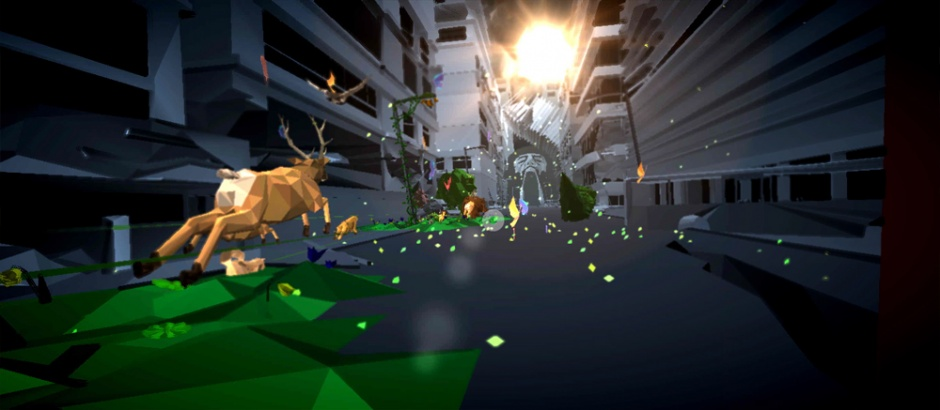
\includegraphics[width=12cm]{summary/rome.jpg}
\end{figure}

\section{Technology}

The browser-based engine is implemented in JavaScript and analyzed in V8 engine. V8 is maintained by Google and is used in the Google Chrome browser. Executable examples are compiled using gcc compiler and are run on the same platform. For additional comparison, the Emscripten project is used to automatically generate JavaScript and measure if the automated conversion may be as effective as writing code by hand.

The project is based on conference sessions and announcements authored by V8 programmers regarding the performance of JavaScript applications. The analysis of available materials is a topic of Chapter 2, where internals of modern engines for dynamic languages are briefly explained.

Chapter 3 covers particles often used to simulate loosely connected systems like smoke, fire, fog, etc. It shows techniques of memory allocation and garbage collection that help improve performance. Two particle systems are presented -- one with high memory allocation that is expected to cause performance issues and the second one, improved by the usage of object pools.

Chapter 4 focuses on sphere collision detection and reaction, with both naive solution and space partitioning using Octree. This benchmark shows an application with high CPU usage and relatively simple math computations. Because of this simplicity, collision detection with spheres is almost always used as a preliminary method of eliminating collision between objects. More complex and expensive algorithms are used to determine the real state of such a pair only if bounding spheres are colliding.

The systems presented in chapters 3 and 4 are not targeted to be full physics engines. They are however representative to general concepts encountered in every game.

Chapter 5 describes Emscripten, a project aimed to convert complete C++ projects to JavaScript. A related library, asm.js, is presented with an overview of architectural choices, which lead to better performance. The generated code is compared to the one created in previous chapters.

The last chapter is a summary of all achieved results. The limitations of JavaScript engines are presented alongside future possibilities for the gaming industry.

Benchmarks are by no means a complete physics system and do not represent the current state of the art of physics algorithms. They are aimed to resemble optimal algorithms in used methods and complexity, so that benchmarks reflect how an actual engine uses memory and computing power.

